\documentclass[a4paper]{article}

\usepackage{amsmath}
\usepackage{amsfonts}
\usepackage{graphicx}
\usepackage{enumerate}
\usepackage{hyperref}
\usepackage{anysize}
\usepackage{hyperref}
\usepackage{listings}
\usepackage{color}
\usepackage{tikz}

\marginsize{2.5cm}{2.5cm}{1.5cm}{1.5cm}
\setlength{\parindent}{0pt}

\graphicspath{{./images/}}

\usetikzlibrary{arrows, shapes}
\tikzstyle{arrow} = [->,font=\scriptsize,>=angle 90]
\tikzstyle{block} = [draw, rectangle, text width=12em, rounded corners, minimum height=2.5em, node distance=1.5cm]
\tikzstyle{cloud} = [draw, ellipse, text width=6em, text centered, minimum height=2.5em]
\tikzstyle{inner} = [inner sep=0, minimum size=0, node distance=1.5cm]

\title{P\&D Encryption---Final Report}
\author{Pieter Maene and Stijn Meul}
\date{\today}

\begin{document}
\lstset{
    language=C,
    numbers=left,
    stepnumber=1,
    numbersep=10pt,
    backgroundcolor=\color{white},
    showspaces=false,
    showstringspaces=false,
    showtabs=false,
    tabsize=2,
    captionpos=b,
    breaklines=true,
    xleftmargin=30pt,
    basicstyle=\footnotesize\ttfamily, 
    breakatwhitespace=true
}

\maketitle

\section{Overview}

\section{Application Description}

The application consists of two main parts: the handshake and the encryption of data packets. For the handshake we use the STS protocol, while the encryption is based on AES-CTR. In this section, we will cover both of them in depth.

\subsection{Handshake}

\begin{center}
    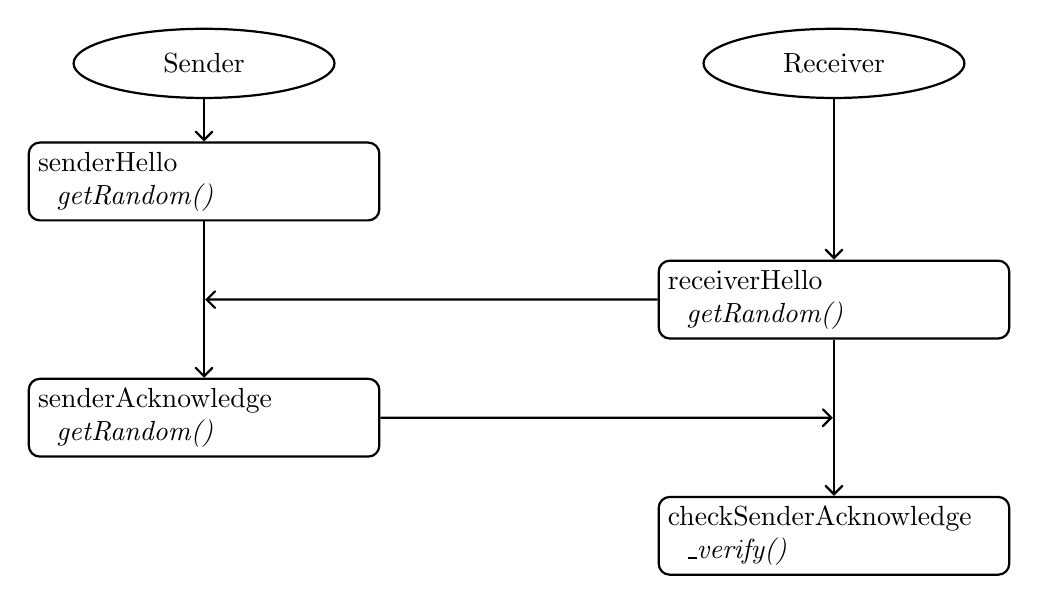
\begin{tikzpicture}[auto, node distance=8cm, thick]
        \node [cloud] (sender) {Sender};
        \node [block, below of=sender] (senderHello) {senderHello\\\textit{\ \ getRandom()}};
        \node [inner, below of=senderHello] (iSenderHello) {};
        \node [block, below of=iSenderHello] (senderAcknowledge) {senderAcknowledge\\\textit{\ \ getRandom()}};
        \node [cloud, right of=sender] (receiver) {Receiver};
        \node [block, below of=receiver, node distance=3cm] (receiverHello) {receiverHello\\\textit{\ \ getRandom()}};
        \node [inner, below of=receiverHello] (iReceiverHello) {};
        \node [block, below of=iReceiverHello] (checkSenderAcknowledge) {checkSenderAcknowledge\\\textit{\ \ \_verify()}};
        
        \path [arrow] (sender) edge (senderHello);
        \path [arrow] (receiver) edge (receiverHello);
        \path [arrow] (senderHello) edge (senderAcknowledge);
        \path [arrow] (receiverHello) edge (iSenderHello);
        \path [arrow] (receiverHello) edge (checkSenderAcknowledge);
        \path [arrow] (senderAcknowledge) edge (iReceiverHello);
    \end{tikzpicture}
\end{center}

\subsubsection{Protocol Messages}
In the Station-to-Station protocol, three messages will be exchanged between the sender and receiver. After this three-way handshake both DSPs will have enough information to calculate two keys (a 128-bit AES key, an 80-bit HMAC key) and a 64-bit nonce used in the CTR mode.

\begin{enumerate}
    \item The sender generates a random number $x$ and then sends $\alpha^x\ mod\ p$ to the receiver. This is shown in Table~\ref{tab:key_exchange_packet_senderhello}.
    \item The receiver generates a random number $y$ and sends $\alpha^y\ mod\ p$ to the sender. We then calculate the RSA signature of the concatenation of $\alpha^y\ mod\ p$ and $\alpha^x\ mod\ p$. This signature is then encrypted using the derived key and nonce. This is shown in Table~\ref{tab:key_exchange_packet_receiverhello}.
    \item The sender acknowledges the message from the receiver by sending its signature to the receiver, using the same procedure described previously. The only difference is that we now concatenate $\alpha^x\ mod\ p$ and $\alpha^y\ mod\ p$. This is shown in Table~\ref{tab:key_exchange_packet_senderacknowledge}.
    \item The receiver checks this final message and verifies the signature. This way, it is able to assert the sender has received correctly too.
\end{enumerate}

\begin{table}[H]
    \begin{center}
        \begin{tabular}{| c | c | c | c | c |}
            \hline
            TAG & KEY \\ \hline\hline
            1B & 156B \\ \hline
            0x00 & $\alpha^x\mod{p}$ \\
            \hline
        \end{tabular}
    \end{center}
    \
    \caption{Key Exchange Packet---SenderHello}
    \label{tab:key_exchange_packet_senderhello}
\end{table}
\begin{table}[H]
    \begin{center}
        \begin{tabular}{| c | c | c | c | c |}
            \hline
            TAG & KEY & SIGNATURE \\ \hline\hline
            1B & 156B & 20B \\ \hline
            0x01 & $\alpha^y\mod{p}$ & $\text{AES}_\text{K}\left(\left(\text{SHA2}\left(\text{PKCS}\left(\alpha^y\small|\alpha^x\right)\right)\right)^{d_R}\mod{n_R}\right)$\\
            \hline
        \end{tabular}
    \end{center}
    
    \caption{Key Exchange Packet---ReceiverHello}
    \label{tab:key_exchange_packet_receiverhello}
\end{table}
\begin{table}[H]
    \begin{center}
        \begin{tabular}{| c | c | c | c | c |}
            \hline
            TAG & KEY & SIGNATURE \\ \hline\hline
            1B & 156B & 20B \\ \hline
            0x02 & $\alpha^y\mod{p}$ & $\text{AES}_\text{K}\left(\left(\text{SHA2}\left(\text{PKCS}\left(\alpha^x \small|\alpha^y\right)\right)\right)^{d_S}\mod{n_S}\right)$\\
            \hline
        \end{tabular}
    \end{center}
    
    \caption{Key Exchange Packet---SenderAcknowledge}
    \label{tab:key_exchange_packet_senderacknowledge}
\end{table}

We decided to use SHA2 instead of SHA3 (which we chose in previous reports) because there is no standardised RSA padding scheme (like PKCS for SHA2) available yet for this hash function. We evualated our RSA implementation using a test vector provided by Mikhail Fomichev and Shayan Kaman Zadeh (Crypto 8).\\

The handshake is rather slow, mainly because there are a lot of modular exponentiations (both in calculating the Diffie-Hellman exponentions and the RSA Sign

\subsubsection{Signature Calculation}

The signature calculation is the part of the handshake that takes the longest. This is because the RSA algorithm requires modular exponentations of large primes. 

\subsection{Data Encryption}

\section{Optimizations}

\subsection{Optimization Table}

\begin{center}
	\begin{tabular}{| l | c | r |}
		\hline
		Code Stage & Number of Cycles & Code Gain \\ \hline
		Base Code & $6,20662313 \cdot 10^{8}$ 	& $0\%$ \\
		CRT Optimization & $4,35591090 \cdot 10^{8}$ & $29,82\%$ \\
		USE64WITH32 Optimization 	& $4,29177952 \cdot 10^{8}$ & $1,03\%$ \\
		Optimization of Conversion Functions & $4,24002677 \cdot 10^{8}$ & $0,83\%$ \\
		Restrict Optimization	 & $1,80351722 \cdot 10^{8}$ & $39,26\%$ \\
		\hline
	\end{tabular}
\end{center}
\subsection{CRT Optimization}
The implementation of the Chinese Remainder Theorem is an algorithmic optimization and not a DSP specific one. 

\subsubsection{Example}
SOME THEORETICAL EXAMPLE HERE

\subsubsection{Impact of the Optimization}

\subsection{USE64WITH32 Optimization}
USE64\_WITH32 is a $\#$define statement in the BigDigits library we are using. If this switch is activated, 64-bit behavior is simulated in 32-bit environment in C.

\subsubsection{Example}
When the USE\_64WITH32 flag is set the following code is called for the multiply function. The performance gain can be seen as there is no seperate code to do the transfer of carry bits from one 32-bit variable to another.

\lstinputlisting[language=C]{source/use64.c}

\subsubsection{Impact of the Optimization}
The impact of this optimization is quite large as the multiply function is called many times during the handshake. This gives an optimization of $1,85071223\cdot10^{8}$ cycles.

\subsection{Optimization of Conversion Functions}
This optimization is more an improvement of our code than a real DSP optimization. The optimization was applied in the handshake functions of the code located in protocol.c.\\

All the contents of the field\_t type (the type we use for packets) are passed as char types even if the functions in the bigdigits library require a digit\_t as input. Before the conversion optimization all these digit\_t variables were first converted from digits to chars using the mpConvToOctets() function in the bigdigits library. The next function in the handshake then reconverted all these chars to digit\_t types using mpConvFromOctets() so they could be used by the bigdigits library.\\

This conversion and reconversion of these large variables are not only cumbersome for the calculation time, they are also very inefficient in memory usage as each average pointer variable is around 150 bytes long and each conversion required a temporary variable as a destination for the conversion.\\

\subsection{Restrict Optimization}
The addition of the restrict keyword in front of all our pointer variables is a real DSP optimization.

\subsubsection{Example}
The only changes that need to be made to implement the restrict optimization is adding the restrict keyword in front of all the pointer arguments in the function headers. An example of a function header with the restric keyword:

\lstinputlisting[language=C]{source/restrictheader.c}
An example of the same function header before the restrict optimization:

\lstinputlisting[language=C]{source/norestrictheader.c}

\subsubsection{Impact of the Optimization}
When the compiler is compiling code with a lot of pointer arguments, it is being very pessimistic about the content of the pointer arguments. For the compiler it is much safer to suppose all the contents of the pointer are changed during the function call except that in most implementations this assumption is too strong. When adding the restrict keyword in front of pointer arguments, the compiler supposes that only the current function is altering the values of the pointer. By doing so the compiler is able to parallelize most of the copying from and to that variable which gives a great improvement.\\

As the average pointer variable in our code has a length of approximately 150 bytes, this optimization results in a much faster execution time. $2,43650955\cdot10^{8}$ cycles are saved by implementing this DSP optimization.

\section{Porting and Integration}

\section{Lessons Learnt}

\section{Conclusions}

\end{document}
